\chapter{Prototype - Development and Implementation\label{cha:prototype}}
%657
This chapter presents design and implementation of the \ep~aided environment
that provides support for \LLLs in universities.

Previous chapters (Chapter \ref{cha:litrev} and \ref{cha:systudy}) identified
recommendations and needs for successful \LLLs support. With the help of the
major stakeholders, Chapter \ref{cha:model} took these highly conceptual
requirements to the practical level of the system features. Now, in this chapter
development of these features using open-source \ep~system Mahara as a basic
platform for implementation is described.

This chapter starts with briefly discussing the overall architecture of the
environment and development toolkit. Then, each implemented component is
presented with its relation to the requested features and \LLLs recommendations
from the literature.

\section{Architecture}

Figure \ref{fig:arch} shows the overall architecture of the environment which
consists of two main components: institutionally controlled LMS and an external,
but institutionally supported \ep~system. Main implementations were carried
out in the \ep~system environment as the features prioritised by the interview
participants were largely in the \ep~domain. They included developing such
components and modules as version control, artifacts' fragments extraction,
concept mapping, timeline based progress tracking and advanced sharing options.

\begin{figure}[htp]
\centering
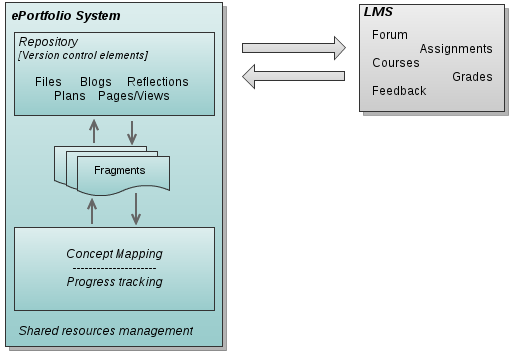
\includegraphics[width=0.8\textwidth]{CH6-F1-Architecture}
\caption{Environment architecture}
\label{fig:arch}
\end{figure}

Each component provided working functionality sufficient to demonstrate the
general concept. Non-functional requirements described in Chapter
\ref{cha:model} were not taken into account as non-essential ones in functional
prototype.

Features that involved LMS environment were not considered for implementation,
as there were enough road-map specifications discovered in the area of
\ep~development that included integration and data transfer between LMS and an
\ep~system. As well, stakeholders did not identified LMS functionality as
important one in \LLLs context. However, LMS was still described in overall
architecture as there were a number of improvements required.

\section{Development Toolkit}

Using Mahara \ep~system as an initial system defined technologies that were
employed in development phase. Development and prototype environments were
installed on LAMP\footnote{\url{http://en.wikipedia.org/wiki/LAMP_(software_bundle)}}
software bundle for Linux which included Apache HTTP Server, MySQL database
server and PHP. These were the basic components for building a general purpose
web server.

The Eclipse\footnote{\url{http://www.eclipse.org}} Platform with PHP Development
Tools\footnote{\url{http://eclipse.org/pdt}} was used for implementation.

Following standards and external packages were used in development:

\begin{itemize}

\item HTML5 + CSS -- standards combined with JavaScript used for drawing
diagrams that represent concept maps, developing a dynamic timeline and
accessing fragments of media (audio/video);

\item jQuery\footnote{\url{http://jquery.com}} -- a JavaScript library that
simplifies HTML document traversing, event handling, animating, and Ajax
interactions for rapid web development;

\item jQuery UI\footnote{\url{http://jqueryui.com}} -- a JavaScript library
built on top of the jQuery for development of highly interactive web applications;

\item jCrop v0.9.9\footnote{\url{http://deepliquid.com/content/Jcrop.html}}
-- jQuery Image Cropping Plugin used in artifacts fragments (Section
\ref{sec:frag});

\item Graphic JavaScript Tree with
Layout\footnote{\url{http://www.codeproject.com/KB/scripting/graphic_javascript_tree.aspx}}
-- a library that allows drawing dynamic concept maps. This library was
significantly modified to meet the needs of the project.
\end{itemize}

Prototype functionality was tested mainly in Google
Chrome\footnote{\url{http://www.google.com/chrome}} v14.0 and Mozilla
Firefox\footnote{\url{http://www.firefox.com}} v4.0 web browsers. Other web
browsers (e.g. Microsoft Internet
Explorer\footnote{\url{http://www.microsoft.com}}) that did not provide native
support for HTML5 elements such as Canvas, required for concept map layout, and
embedded video/audio, used in artifact's fragments, were not used in testing.

\section{Implementations}

Components added to the standard Mahara \ep~installation were expected to
address the requirements developed by the stakeholders and derived from the
literature review.

Table \ref{tab:implement} matches implemented components to the requested
features.

\begin{center} \small
    \tablefirsthead{
     \hline
     \multicolumn{1}{|c|}{\textbf{Component}} &
     \multicolumn{1}{c|}{\textbf{Feature}} \\
     \hline}
    \tablehead{
     \hline
     \multicolumn{2}{|l|}{\small\sl continued from previous page}\\
     \hline
     \multicolumn{1}{|c|}{\textbf{Component}} &
     \multicolumn{1}{c|}{\textbf{Feature}} \\
     \hline} 
    \tabletail{
     \hline
     \multicolumn{2}{|r|}{\small\sl continued on next page}\\
     \hline}
    \tablelasttail{\hline} 
	\bottomcaption{Implemented \ep~system components}
    \begin{supertabular}{| p{6cm} | p{6cm} |}
    Version control elements & \\ \hline
    Concept mapping module & \\ \hline
    Artifacts' fragments extraction & \\ \hline
    Learning progress tracking & \\ \hline
    Advanced sharing options & \\ \hline
    \end{supertabular}
    \label{tab:implement}
\end{center}

\subsection{Version Control Elements}

Screenshots for every feature.

\subsection{Concept Mapping Module}

Addressing the challenges of \ep~knowledge management\footnote{In this thesis,
the \ep~knowledge management is referred to in terms of creating knowledge,
sharing it, managing and organizing it in \ep~space.} and development of
graduate attributes, that represent the core learning outcomes, skills and
qualities that students should develop during their university education, as
have for example been outlined in \citet{Hughes2010}, was a complex problem
which required a creative approach and no clearly suggested solution from the
stakeholders. While looking at the other areas for potential solution, it was
discovered that qualitative data analysis and knowledge visualization using
concept mapping tool have properties suitable for \ep~domain. Like \ep~work,
qualitative data analysis is characterised by rich data sets, opening the
possibility of borrowing well established techniques. Concept maps had potential
as a supporting tool for organizing these data sets into concepts and
visualising them in a way that could be understood by relevant audiences.

This section describes how bringing these two techniques together helped to
develop a solution for the problems outlined earlier.

\subsubsection{Parallels to qualitative research}

An \ep~can be called a container that needs to be organized, with students not
always knowing which items to select and where the items they put in their
\ep~should go. Students start their \ep~work by collecting \textit{raw} data
available from formal learning and outside activities and transforming it into
information that they decide to put into their \ep. After working with and
reflecting on this information students arrive at knowledge. A parallel with
qualitative data analysis can be drawn here where researchers either develop new
theories from data, moving from specific observations to general concepts and
theories (inductive approach), or they try to check if their data map against
the theories that are already known and understood (deductive approach)
\citep{Strauss2008,Patton2002}. An assumption here is that analyzing one's own
learning process takes similar steps as qualitative data analysis: small bits,
specific data that learners are collecting, contribute to the bigger picture of
knowledge development. The difference is that the learner developing their
\ep~is not aware of the existing theories yet. These theories are the concept
structures that exist in the understanding of society, institution and
employers. However, these must be eventually understood and \textit{made their
own} by the learner. Like the qualitative researcher, the learner needs to
immerse themselves in their data and to come to an understanding of the kind of
material they should be collecting in their \ep~and the concepts that express
their learning goals. They need to find (and to a certain degree construct by
exposing themselves to learning opportunities) evidence in their data to show
that they conform to these concepts.

In qualitative research, a number of techniques are available to the researcher
in managing, analyzing and interpreting their data, such as coding, grouping,
generating categories and themes, rearranging and sorting \citep{Marshall2010}.
To support these techniques, specialized qualitative data analysis software
(QDAS), like
NVivo\footnote{\url{http://www.qsrinternational.com/products_nvivo.aspx }} and
MAXQDA\footnote{\url{http://www.maxqda.com}}, has been developed which largely
allows coding, linking and mapping unstructured information. Although, QDAS
could provide students with necessary functionality for data analysis, it cannot
substitute the role of an \ep~system in the learning process. Reasons for
that are outlined in Table \ref{tab:qdas}.

\begin{table}[htb]
  \begin{center}
    \begin{tabular}{| p{6cm} | p{6cm} |}
    \hline
     \multicolumn{1}{|c|}{\textbf{QDAS}} &
     \multicolumn{1}{c|}{\textbf{\ep~system}} \\
     \hline
     Help researchers to understand data & Help students to understand data and
     theories \\ \hline 
     Develop codes, concepts and theories; visualize relations between concepts
     & Showcase students' growing understanding of theories and their data \\
     \hline 
     Produce a report as an end point of the research  & Does not have an end
     point; data is constantly evolving; old concepts are changing and new are
     emerging with changing understanding of these concepts \\ \hline 
    \end{tabular}
  \end{center}
  \caption{Conceptual difference between QDAS and \ep~system}
  \label{tab:qdas}
\end{table}

However, the strength of QDAS is in how it allows to work closely with data.
Researchers \textit{label} data with codes, not just in order to connect these
labels later, but as an opportunity to \textit{dive} into their data by
re-reading, listening or watching it over and over again. This strength is
important for students as they need to revisit their material as their
understanding of concepts grows.

Currently, the majority of \ep~systems allow tagging their content with
user-defined tags. However, according to the results of interviews with
students, tagging does not provide necessary meaning to the \ep~data,
cannot show relations between concepts and does not allow building a flexible
structure. To address this problem, concept mapping was introduced into
\ep~environment to help students to be able use the same techniques available in
qualitative data analysis to manage unstructured data and develop learning
concepts in their \ep.

\subsubsection{Concept maps}

\citet{Mcaleese1998} formally defines a concept map as a directed acyclic graph
that consists of a set of Concept Labels and a non-empty set of Relationships
between Concepts. Putting it simply, concept maps are graphical representation
of the hierarchy of knowledge concepts and connections between them
\citep{Novak2008}.

Concept maps fit well with the qualitative data analysis techniques, outlined in
the previous section, as they are dynamic, process-oriented and give learners an
opportunity to engage in the learning process \citep{Mcaleese1998} which is
important for \LLLs \citep{Schuetze2006,Divjak2004}. Maps are created over time
by the learner who is engaged in a process of reflection, collecting and
selecting appropriate examples of their work. With concept maps learners can
interpret their personal knowledge and map this knowledge and individual
examples against the existing theories. The hierarchical nature of the concept
map allows for organizing concepts from the high level abstract concept to the
more specific concepts. This property can be used by students for managing and
structuring data in their \ep s. In addition, while describing future directions
for \ep~technology, Cambridge \citeyearpar{Cambridge2010} suggested that
visualization in the form of concept maps could be a potential way of generating
reflections.

QDAS already offers tools similar to concept maps in form of textual hierarchies
of nodes/terms/labels/concepts or as diagrams that show relations between
labels. Adding concept maps functionality to an \ep~system might make it
possible to borrow well established techniques of qualitative data analysis and
help students, who are analyzing their learning, to formally do what QDAS
already does informally. 

Concept maps have been already successfully used to in education to communicate
complex ideas, assess understanding of learning objectives, elicit knowledge and
provide conceptual frame for learning \citep{Novak2010}. A complete review of
the concept maps is beyond the scope of this thesis. For detailed examples and
evaluation of effectiveness of this tool refer to The Institute for Human and
Machine Cognition research group report \citep{Canas2003}.

\subsection{Artifacts' Fragments Extraction}
\label{sec:frag}

This would allow the presentation of different artifacts to different audiences,
but at the same time saving duplication of materials as all artifacts will be
hosted together. 

From the perspective of this component evolving Media Fragments 1.0
specification \citep{MediaGroup2011} becomes very useful as it describes the
ways of extracting temporal and spatial media fragments using Uniform Resource
Identifiers (URI). Once it is finished, this specification could be adopted in
the \ep~system for improved fragments description and extraction.

\subsection{Learning Progress Tracking}

\subsection{Advanced Sharing Options}

What was added: history, re-share, notifications, share by email.

\section{Prototype Iterations and User Tests}
 
Before formal evaluation was undertaken, implemented functionality had been
tested by users. Overall, time and resources constraints of the project allowed
for two planned prototype iterations. Each iteration produced a workable version
of the implemented features. At the end of each iteration, the functional
prototype was presented to a student and a lecturer selected from the
participants of the requirements elicitation phase who had agreed to continue
their participation in this research.

Each feedback session included up to an hour demonstration and discussion of the
implemented functionality. Users were encouraged to give their ideas about
potential improvements and 

Feedback between iterations was very useful as it provided information on
necessary improvements and drawbacks of current implementations. Users were
generally satisfied with the improvements and made largely positive comments.
However, several issues were noted: \ldots

All discovered issues were addressed in the later versions of the prototype
in preparation for the formal evaluation stage.

\section{Summary}

This chapter presented \ldots